\section{Zielsetzung}
In diesem Versuch wird die Erzeugung freier Elektronen mithilfe des glühelektrischen Effektes untersucht. Es werden Kennlinien der verwendeten Hochvakuumdiode 
analysiert und die Austrittsarbeit der Elektronen aus dem Kathodenmaterial (Wolfram) bestimmt.

\section{Theorie}
\label{sec:Theorie}
Metalle besitzen \textit{Leitungselektronen}, welche an kein Atom gebunden sind und sich frei in dem Metall bewegen können. Das Gesamtpotential der ionisierten Atome
ist näherungsweise konstant in dem Leiter und ist um den Betrag $\phi$ verschieden zum Potential des Außenraumes. Die Elektronen befinden sich folglich in einer Art 
Potentialtopf, dessen (Energie-)Barrieren sie überwinden müssen, um aus dem Material austreten zu können. Eine schematische Darstellung der Situation ist \autoref{fig:Potentialtopf}
zu entnehmen.

\begin{figure}
    \centering
    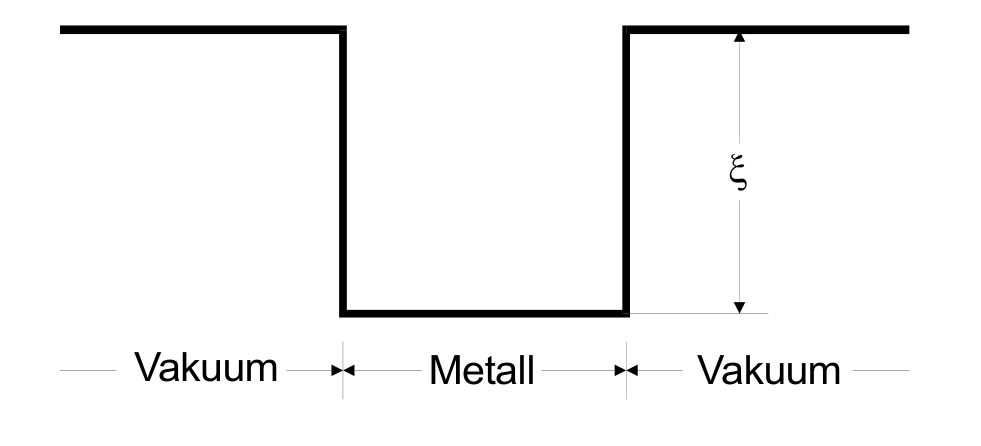
\includegraphics[width = 0.5\textwidth]{content/Potentialtopf.png}
    \caption{Potentialtopfmodell des Elektrons im Metall \cite{v504}.}
    \label{fig:Potentialtopf}
\end{figure}

Aus der Quantenmechanik folgt, dass die Elektronen nur diskrete Energiewerte $E_n$ annehmen können. Das \textit{Pauli-Verbot} besagt, dass jeweils nur zwei Elektronen 
mit entgegengesetztem Spin den gleichen Energiewert annehmen können. Dies bedeutet, dass zu jeder Temperatur Elektronen unterschiedlicher Energien existieren. 
Auch beim absoluten Nullpunkt $T = 0$ exisitieren so Elektronen, welche die maximale Energie $\zeta$ besitzen. Die Wahrscheinlichkeit, dass sich ein Elektron 
in einem Zustand mit der Energie $E$ befindet wird durch die \textit{Fermi-Diracsche Verteilungs-Funktion} beschrieben, welche sich für die in diesem Versuch erreichten 
Temperaturbereiche zu 
\begin{equation}
    \label{eqn:Fermi_Dirac}
    f(E) \approx \mathrm{exp}\left( \frac{\zeta - E}{kT} \right)
\end{equation}
vereinfacht.

\subsection{Glühelektrischer Effekt und Hochvakuumdiode}
\label{subsec:Glueelek}
Da eine höhere Temperatur eine höhere kinetische Energie der Elektronen bedingt, können mehr Elektronen aus einem Kathodenmaterial austreten, je heißer dieses ist.
Bei der Erzeugung freier Elektronen mithilfe einer Hochvakuumdiode wird dieser Effekt ausgenutzt. Die Glühkathode wird über einen Heizstrom $I_\text{H}$ aufgeheizt,
sodass ausreichend Elektronen die Austrittsarbeit überwinden und das Material verlassen können. Über eine Beschleunigungsspannung (Saugspannung) $U_\text{B}$
wird ein elektrisches Feld zwischen Kathode und einer Anode erzeugt, in welchem die nun freien Elektronen in Richtung Anode beschleunigt werden. 
In der Diode herrscht ein Hochvakuum, wodurch ein Wechselwirken der Elektronen mit Gasmolekülen vermieden wird.
Der Aufbau einer solchen Diode und die Polung der Spannungen ist \autoref{fig:Hochvakuumdiode} zu entnehmen.
\begin{figure}
    \centering
    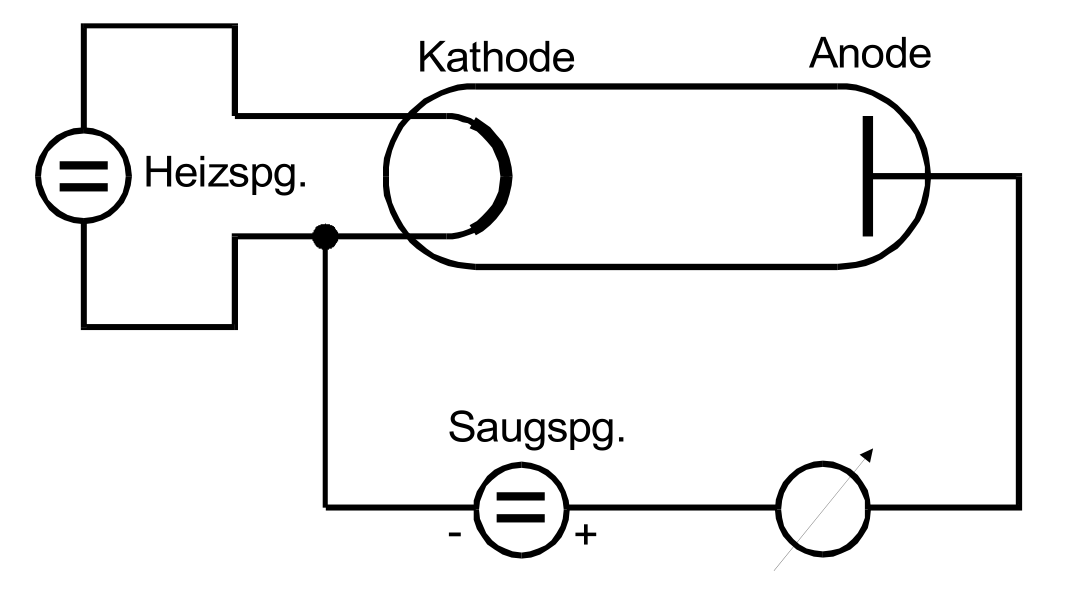
\includegraphics[width = .5\textwidth]{content/Vakuumdiode.png}
    \caption{Aufbau einer Hochvakuumdiode \cite{v504}.}
    \label{fig:Hochvakuumdiode}
\end{figure}

\subsection{Kennlinie der Hochvakuumdiode}
\label{subsec:T_Kennlinie}
Wird der Anodenstrom $I$ gegen die Beschleunigungsspannung $U_\text{B}$ aufgetragen, ergibt sich ein typischer Kurvenverlauf, der sich in verschiedene Bereiche 
unterteilen lässt, die in diesem Versuch untersucht werden. Die Kennlinie einer Hochvakuumdiode und die Unterteilung der Bereiche sind in \autoref{fig:Kennlinie} abgebildet.

\begin{figure}
    \centering
    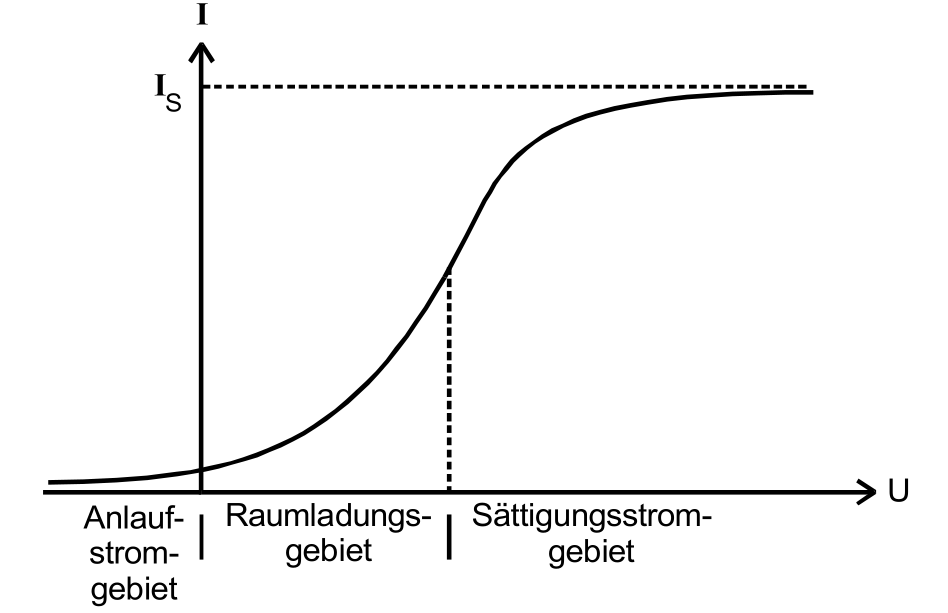
\includegraphics[width = .5\textwidth]{content/Kennlinie.png}
    \caption{Kennlinie einer Hochvakuumdiode und Unterteilung in wichtige Bereiche des Stroms \cite{v504}.}
    \label{fig:Kennlinie}
\end{figure}

\subsubsection{Sättigungsstrom}
Der Sättigungsstrom beschreibt den Strom, der bei einer gegebenen Temperatur maximal erreicht werden kann. Er stellt sich ein, sobald das Raumladungsgebiet in \ref{fig:Hochvakuumdiode}
überwunden ist. Um den Sättigungsstrom zu ermitteln wird betrachtet, wie viele Elektronen über die zum Austritt mindestens nötige Energie 
$\zeta + e \cdot \phi$ ($e$: Elementarladung) verfügen. Durch Beachtung der quantenmechanischen Eigenschaften der Elektronene und Verwendung der \autoref{eqn:Fermi_Dirac} ergibt sich
für den Strom aus dem Kathodenmaterial

\begin{equation}
    \label{eqn:J_S}
    j_\text{S}(T) = 4 \symup{\pi}\frac{e m_0 k^2}{h^3}T^2 \cdot \symup{e}^{-\frac{e\phi}{kT}},
\end{equation}
wobei $k$ die Boltzmannkonstante, $h$ das Plancksche-Wirkungsquantum und $m_0$ die Ruhemasse des Elektrons ist. Die an der Anode messbare Stromstärke berechnet sich mit der 
emmitierenden Kathodenoberfläche $f$ zu $I_\text{S} = j_\text{S} \cdot f$.

\subsubsection{Raumladungsgebiet}
Bei der Beobachtung der Kennlinie einer Diode kann festgestellt werden, dass bevor der Sättigungsstrom $I_\text{S}$ erreicht wird, der Anodenstrom eine Abhängigkeit zur 
Beschleunigungsspannung aufweist. Dies hat die Ursache, dass bei geringen Beschleunigungsspannungen nicht alle Elektronen die Anode erreichen. Die Kontinuitätsgleichung
besagt, dass $j = -\rho \cdot v$ gilt, wobei $j$ der Strom, $\rho$ die Raumladungsdichte und $v$ die Geschwindigkeit der Elektronen ist. Da die Geschwindigkeit der Elektronen auf Grund
der Beschleunigung nicht kosntant ist, aber der Strom $j$ sehrwohl, ergibt sich, dass die Raumladungsdichte $\rho$ eine Funktion des Ortes sein muss.
Die Raumladungsdichte ist somit nicht homogen und beeinflusst den Verlauf der Feldlinien des elektrostatischen Feldes zwischen Kathode und Anode. 
Da so das elektrische Feld vor der Kathode teilweise abgeschirmt wird, werden nicht alle ausgelösten Elektronen von diesem erfasst, was einen geringeren Anodenstrom zur Folge hat.
Aus einer Potentialbetrachtung geht hervor, dass der Strom im Bereich des Raumladungsgebiets der Gleichung
\begin{equation}
    \label{eqn:Raumladung}
    j = \frac{4}{9}\varepsilon_0 \sqrt{\frac{2e}{m_0}}\frac{V^{3/2}}{a^2}
\end{equation}
genügt. Dies ist die \textit{Langmuir-Schottkysche Raumladungsgleichung}. 
Wie sich erkennen lässt, besteht eine Abhängigkeit zur Beschleunigungsspannung $U$ mit dem Exponenten $3/2$. $a$ ist der Abstand von Anode und Kathode.

\subsubsection{Anlaufstrom}
Selbst bei einer Beschleunigungsspannung von $U_\text{B} = 0$ und sogar negativen Werten dieser (entgegengesetzte Polung) lässt sich ein geringer Anodenstrom beobachten.
Dies ist damit zu erklären, dass die Elektronen beim Austritt aus der Kathode eine gewisse kinetische Energie besitzen, die es ihnen ermöglicht gegen die Beschleunigung
eines Gegenfeldes die Anode zu erreichen.
Es ergibt sich, dass der Strom exponentiell vom äußeren Potential $V$ gemäß
\begin{equation}
    \label{eqn:j_Anlauf}
    j(V) = j_0 \mathrm{exp}\left(-\frac{e\phi_\text{A} + e \cdot V}{kT} \right) = const \cdot \mathrm{e}^{-\frac{e \cdot V}{kT}}
\end{equation}
abhängt.

\subsection{Temperaturberechnung der Kathode}
\label{subsec:Temperatur_Kathode}
Die Strahlungsleistung der Diode lässt sich mithilfe des \textit{Stefan-Boltzmann'schen Gesetzes} zu 
\begin{equation*}
    N_\text{Str} = f \eta \sigma T^4
\end{equation*}
berechnen. Für die \textit{Stefan-Boltzmannkonstante} gilt $\sigma = \qty{5.7e-12}{\watt\per\centi\metre\squared\kelvin^4}$ \cite{scipy}. $\eta$ ist der Emissionsgrad
der Kathode. Wenn die Wärmeleistung $N_\text{WL}$ der Kathode bekannt ist, ergibt sich mit der zugeführten Leistung $N_\text{zu} = U \cdot I$ die Bilanz
\begin{equation}
    \label{eqn:Leistung}
    U \cdot I = f \eta \sigma T^4 - N_\text{WL}
\end{equation} 
für die Leistungen der Kathode, woraus sich die Temperatur $T$ der Kathode bestimmen lässt.
